\section{516 --- Longest Palindromic Subsequence (LeetCode)}

\subsection*{Código}
\lstinputlisting{516_LongestPalindromicSubsequence.java}

\subsection*{Comprovante de aceite}
\begin{center}
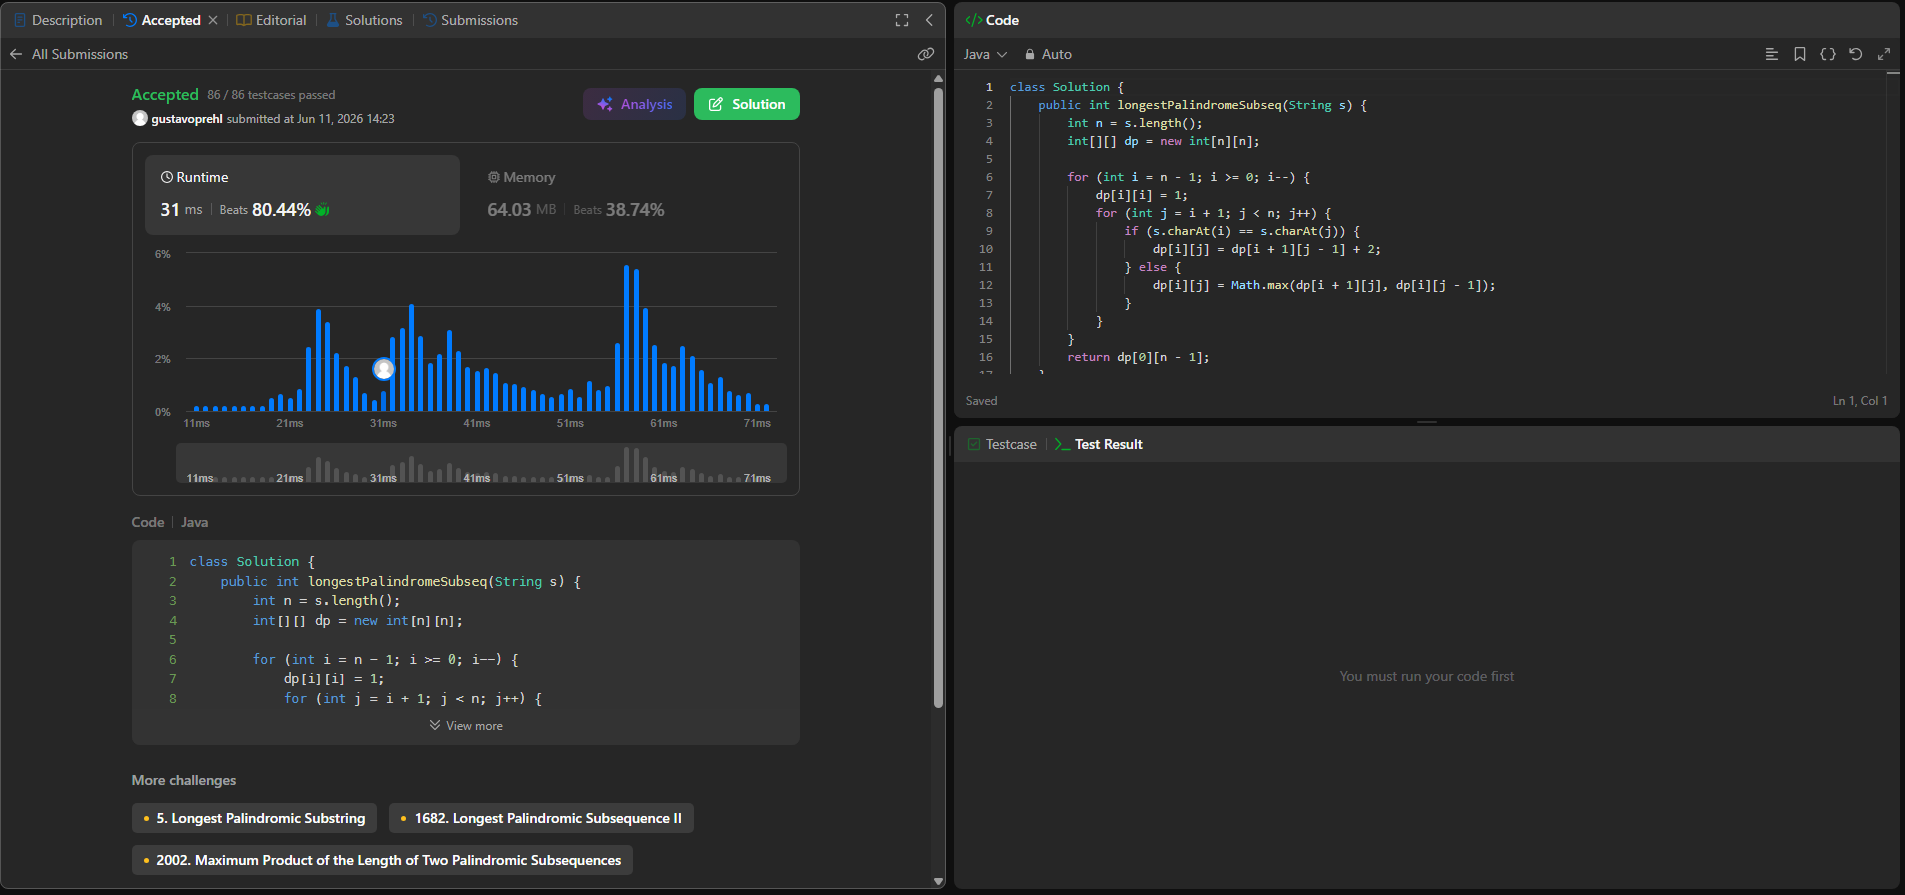
\includegraphics[width=0.85\textwidth]{Accepts/516_LongestPalindromicSubsequence_Submit.png}\\
\end{center}

\subsection*{Justificativa}

\textbf{Estratégia:} programação dinâmica em intervalos (\emph{interval
DP}).

\textbf{Definição do subproblema:} \texttt{dp[i][j]} representa o
comprimento da maior subsequência palíndroma contida em \texttt{s[i..j]}
(substring de \texttt{i} a \texttt{j}, inclusive).

\textbf{Subestrutura ótima (recorrência):} compara-se os caracteres das
extremidades do intervalo:
\begin{itemize}
    \item Se \texttt{s[i] == s[j]}, ambos os caracteres podem fazer parte da
    subsequência palíndroma (um na ponta esquerda, outro na direita), e o
    problema se reduz a encontrar a maior subsequência palíndroma do
    intervalo interno \texttt{s[i+1..j-1]}, somando 2:
    \texttt{dp[i][j] = dp[i+1][j-1] + 2}.
    \item Se \texttt{s[i] != s[j]}, pelo menos um dos dois extremos não pode
    pertencer à subsequência ótima, então a resposta é o melhor entre
    ignorar a extremidade esquerda ou a direita:
    \texttt{dp[i][j] = max(dp[i+1][j], dp[i][j-1])}.
\end{itemize}

\textbf{Caso base:} \texttt{dp[i][i] = 1}, pois um único caractere é sempre
um palíndromo de tamanho 1.

\textbf{Subproblemas sobrepostos e ordem de preenchimento:}
\texttt{dp[i][j]} depende apenas de subintervalos menores
(\texttt{dp[i+1][j-1]}, \texttt{dp[i+1][j]}, \texttt{dp[i][j-1]}), todos com
\texttt{i} maior ou \texttt{j} menor que o intervalo atual. Preenchendo
\texttt{i} de \texttt{n-1} até \texttt{0} e, para cada \texttt{i},
\texttt{j} de \texttt{i+1} até \texttt{n-1}, garante-se que toda dependência
já foi calculada antes de ser usada (programação dinâmica \emph{bottom-up}).

\textbf{Resposta final:} \texttt{dp[0][n-1]}, o intervalo que cobre a string
inteira.

\textbf{Complexidade:}
\begin{itemize}
    \item Tempo: $O(n^2)$, um valor para cada par $(i, j)$ com
    $i \leq j$.
    \item Espaço: $O(n^2)$ para a tabela \texttt{dp}.
\end{itemize}

\textbf{Tópico do curso:} \emph{Programação Dinâmica} [CLRS09, cap. 15] ---
formulação de \texttt{dp[i][j]} sobre intervalos da string, com recorrência
baseada em subintervalos menores e preenchimento \emph{bottom-up} respeitando
as dependências entre subproblemas.
